\documentclass[11pt,a4paper]{article}
\usepackage[margin=2.3cm]{geometry}
\usepackage[T1]{fontenc}
\usepackage{graphicx,booktabs,float,caption,array,amsmath}
\usepackage[table]{xcolor}
\usepackage{listings}
\usepackage{tikz}
\usetikzlibrary{positioning,arrows.meta,shapes.geometric,fit,backgrounds}
\usepackage[hidelinks]{hyperref}

\graphicspath{{../figures/}{figures/}{./}}
\captionsetup{font=small,labelfont=bf}
\setlength{\parskip}{0.4em}
\setlength{\parindent}{0pt}

\lstset{basicstyle=\ttfamily\footnotesize,breaklines=true,frame=single,
  keywordstyle=\bfseries,columns=fullflexible,xleftmargin=0pt,
  language=Python,showstringspaces=false,backgroundcolor=\color{gray!6}}

\definecolor{sparkorange}{HTML}{E25A1C}
\definecolor{blue1}{HTML}{2A6FB0}

\title{\textbf{Scalable Analysis of 1.39 Million Lichess Chess Games\\with Apache Spark and PySpark}}
\author{Mining of Massive Datasets --- Assignment 2 (Group)\\[2pt]
\small Group members: \textit{[add names / roll numbers]}}
\date{}

\begin{document}
\maketitle

\begin{abstract}
We build a scalable data-processing pipeline in Apache Spark (PySpark) over a real-world
dataset of \textbf{1,389,994 rated chess games} from the open Lichess database
(December 2013 -- February 2014; 93.3 million half-moves, 36,666 distinct players).
The pipeline parses the raw PGN dump into a flat table, loads it with RDDs
(\texttt{map}, \texttt{filter}, \texttt{flatMap}, \texttt{reduceByKey}), cleans and
analyses it with DataFrames and Spark SQL, chains both into a documented
RDD$\rightarrow$DataFrame workflow, and finally replays 200,000 games as a live feed
through Spark's micro-batch streaming engine. Results include the most played openings,
the effect of time control on game length and termination, white's first-move advantage
(52.5\% score), a monotone relationship between rating gap and upset probability
(44\% for equal players, 10\% for gaps over 400 points) and the observation that draws
become more than twice as frequent between 1000- and 2200-rated players. We also
report an honest account of the platform limits met on Windows, notably that
Structured Streaming could not be executed locally, so the streaming results come from
Spark's DStream micro-batch API.
\end{abstract}

%------------------------------------------------------------------
\section{Introduction}
Chess servers produce a continuous stream of small, structured, but very numerous
records: one game is a few hundred bytes, yet Lichess completes hundreds of thousands to millions every month.
This makes game logs a good fit for the data-parallel model taught in the course:
the records are independent, the useful questions are aggregations (counts, averages,
group-bys), and the data naturally arrives as a stream. We use Apache Spark to answer
such questions at a scale that a single-threaded script handles poorly.

The objectives, mapped to the assignment parts, are:
\begin{itemize}\itemsep0pt
\item \textbf{A} --- prepare a Spark environment and explain its architecture;
\item \textbf{B} --- load the data with RDDs and apply transformations and actions;
\item \textbf{C} --- build DataFrames, clean, query, and use Spark SQL;
\item \textbf{D} --- document an Input$\rightarrow$RDD$\rightarrow$DataFrame$\rightarrow$Output workflow;
\item \textbf{E} --- simulate a stream, process incoming records, and aggregate per batch;
\item \textbf{F} --- consolidate everything in this report.
\end{itemize}
All code, results and figures are in the accompanying repository
(\texttt{src/}, \texttt{results/}, \texttt{figures/}).

%------------------------------------------------------------------
\section{Dataset Description}
\textbf{Source.} The Lichess Open Database
(\url{https://database.lichess.org}) publishes every rated game as monthly PGN files
compressed with Zstandard. We use \texttt{lichess\_db\_standard\_rated\_2014-01} and
\texttt{...2014-02} (111~MB and 113~MB compressed, 698k and 692k games).
Because the UTC timestamps of the first January games fall on 31 December 2013, the data
spans 31 Dec 2013 -- 28 Feb 2014.

\textbf{Preparation.} PGN is a multi-line text format that Spark cannot split into records
natively, so \texttt{src/parse\_pgn.py} streams the compressed file, extracts tags,
strips comments and move numbers, and writes one CSV row per game. The two months were
merged and de-duplicated on game id, giving the \textbf{1,389,994-row, 533~MB} table
used throughout (the requirement was at least 10k).

\begin{table}[H]\centering\small
\caption{Attributes of the game table (16 columns).}
\begin{tabular}{@{}lll@{}}\toprule
Attribute & Type & Description\\\midrule
\texttt{game\_id} & string & Lichess game identifier (unique key)\\
\texttt{white}, \texttt{black} & string & Player user names\\
\texttt{result} & category & \texttt{1-0}, \texttt{0-1} or \texttt{1/2-1/2}\\
\texttt{white\_elo}, \texttt{black\_elo} & int & Players' ratings before the game\\
\texttt{white\_diff}, \texttt{black\_diff} & int & Rating change caused by the game\\
\texttt{eco}, \texttt{opening} & string & ECO code (A00--E99) and opening name\\
\texttt{time\_control} & string & \texttt{base+increment} in seconds, e.g.\ \texttt{60+0}\\
\texttt{termination} & category & Normal, Time forfeit, Rules infraction\\
\texttt{utc\_date}, \texttt{utc\_time} & string & Start of the game (UTC)\\
\texttt{num\_moves} & int & Half-moves (plies) played\\
\texttt{moves} & text & Space-separated move list in SAN\\\bottomrule
\end{tabular}\end{table}

\textbf{Type of data.} Multi-dimensional records with a free-text component (the move
list is a ``document'' of 67 tokens on average, 93.3M tokens in total) and an implicit
player--player graph. Per record the data is small, but the \emph{count} is what makes
it a big-data workload.

\textbf{Applications.} Opening-book and training tools; matchmaking and rating-system
calibration; fair-play and cheat detection; understanding when and how people play, to
size server capacity. The questions we answer in Sections~\ref{sec:rdd}--\ref{sec:df}
are of exactly this kind.

%------------------------------------------------------------------
\section{Spark Architecture and Environment}
\textbf{Environment.} Python 3.11, PySpark 3.5.3, OpenJDK 17, Windows 11, run in
\emph{local mode} (\texttt{local[*]}, 24 logical cores, 6~GB driver memory).
Local mode runs every component inside one JVM but uses the same APIs and execution
model as a cluster, so the code scales out unchanged.

\begin{figure}[H]\centering
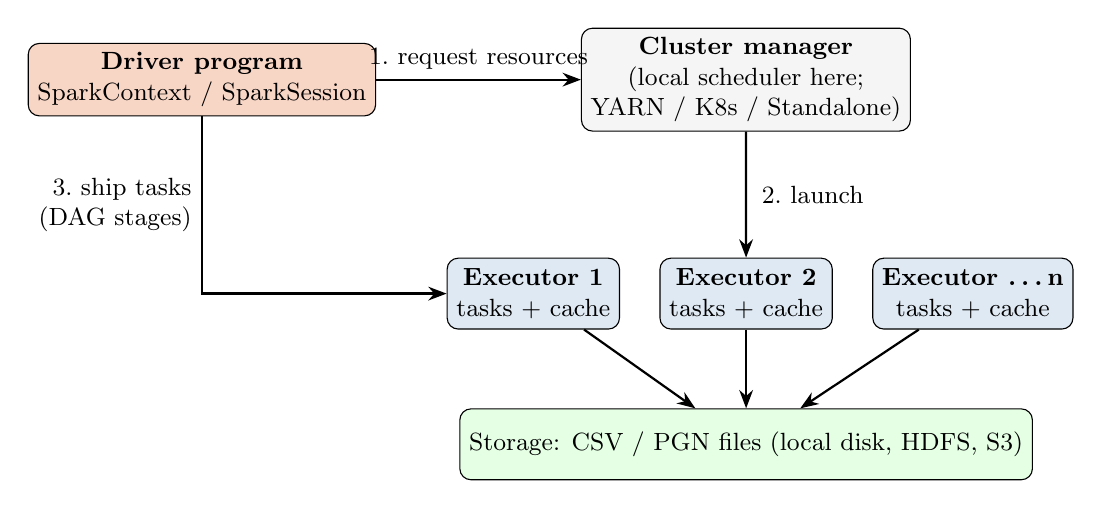
\begin{tikzpicture}[font=\small,
  box/.style={draw,rounded corners,align=center,minimum height=0.9cm,fill=gray!8},
  big/.style={draw,rounded corners,dashed,inner sep=7pt},
  arr/.style={-{Stealth},thick}]
\node[box,fill=sparkorange!25,minimum width=3.6cm] (drv) {\textbf{Driver program}\\SparkContext / SparkSession};
\node[box,right=2.6cm of drv,minimum width=3cm] (cm) {\textbf{Cluster manager}\\(local scheduler here;\\YARN / K8s / Standalone)};
\node[box,below=1.6cm of cm,xshift=-2.7cm,fill=blue1!15] (e1) {\textbf{Executor 1}\\tasks + cache};
\node[box,right=0.5cm of e1,fill=blue1!15] (e2) {\textbf{Executor 2}\\tasks + cache};
\node[box,right=0.5cm of e2,fill=blue1!15] (e3) {\textbf{Executor \dots n}\\tasks + cache};
\node[box,below=1.0cm of e2,minimum width=7cm,fill=green!10] (st) {Storage: CSV / PGN files (local disk, HDFS, S3)};
\draw[arr] (drv) -- node[above]{1.\ request resources} (cm);
\draw[arr] (cm) -- node[right,xshift=2pt]{2.\ launch} (e2);
\draw[arr] (drv) |- node[near start,left,align=right]{3.\ ship tasks\\(DAG stages)} (e1.west);
\draw[arr] (e1) -- (st); \draw[arr] (e2) -- (st); \draw[arr] (e3) -- (st);
\end{tikzpicture}
\caption{Spark architecture. In this project the driver and executors are threads of one
local JVM; the cluster manager is Spark's built-in local scheduler.}
\end{figure}

\textbf{Components.}
The \emph{driver program} holds the \texttt{SparkSession}, turns our transformations into a
DAG, splits it into stages at shuffle boundaries and schedules tasks.
The \emph{cluster manager} allocates executors (local scheduler here).
\emph{Executors} run tasks on data partitions and cache partitions in memory.
\textbf{Workflow of an application:} (1)~the driver creates the session;
(2)~transformations such as \texttt{map} or \texttt{filter} are \emph{lazy} and only extend
the lineage; (3)~an \emph{action} (\texttt{count}, \texttt{collect}, \texttt{takeOrdered})
triggers a \emph{job}; (4)~the job is split into stages at wide dependencies
(\texttt{reduceByKey}, \texttt{groupBy}); (5)~each stage runs one task per partition;
(6)~results return to the driver. The 558~MB CSV was read as 24 partitions.
The \texttt{part\_d\_pipeline.py} run triggered 7 jobs.

\textbf{APIs.} We use all three levels: the low-level RDD API (Section~\ref{sec:rdd}),
DataFrames/Spark SQL with the Catalyst optimiser (Section~\ref{sec:df}), and streaming
(Section~\ref{sec:stream}).

%------------------------------------------------------------------
\section{RDD-Based Processing (Part B)}\label{sec:rdd}
The CSV was loaded with \texttt{sc.textFile} (24 partitions, 1,389,995 lines including
the header) and parsed with the \texttt{csv} module (opening names contain commas).
\begin{lstlisting}
rows = (lines.filter(lambda l: not l.startswith("game_id,"))      # filter
             .map(lambda l: next(csv.reader([l]))))               # map
opening_freq = rows.map(lambda r: (r[9], 1)).reduceByKey(add)     # product-frequency analogue
move_freq = (rows.flatMap(lambda r: r[15].split())                # flatMap: word count
                 .map(lambda m: (m.rstrip("+#"), 1)).reduceByKey(add))
players = rows.flatMap(lambda r: [(r[1],1),(r[2],1)]).reduceByKey(add)
\end{lstlisting}
Actions used: \texttt{count}, \texttt{sum}, \texttt{takeOrdered}, \texttt{collectAsMap}.
The full job set took 275 s on one laptop; the RDD is cached after parsing.

\begin{table}[H]\centering\small
\caption{RDD results over all 1,389,994 raw games.}
\begin{tabular}{@{}p{3.6cm}p{11.8cm}@{}}\toprule
Analysis & Output (top entries)\\\midrule
Opening frequency (2,636 distinct) & Van't Kruijs Opening 41,190; Horwitz Defense 27,499; Modern Defense 27,203; Owen Defense 23,675; Scandinavian: Mieses-Kotroc 22,997\\
Move word count (93,334,516 tokens) & O-O 1,707,127; Nf3 1,349,797; e4 1,299,386; d4 1,218,674; Nf6 1,206,276; e5 1,178,241\\
First move & e4 823,698 (59.3\%); d4 334,633 (24.1\%); e3 46,150; c4 39,241; Nf3 34,758\\
Most active players (36,666 distinct) & ZMAJ 5,697; ribarisah 5,438; 147a 4,380; speedyG 4,338; amir51 3,948\\
Results & 1-0: 707,167 (50.9\%); 0-1: 638,037 (45.9\%); draws: 44,790 (3.2\%)\\
Termination & Normal 931,572; Time forfeit 458,266; Rules infraction 156\\
\texttt{filter}: decisive games, rating gap $\ge$300 & 165,249 games; the lower-rated player won 23,018 (13.9\%)\\\bottomrule
\end{tabular}\end{table}

\textbf{Observations.} The 1.e4 opening is 2.5$\times$ as popular as 1.d4. White wins
5 percentage points more often than black. Move counts are heavy-tailed: a few
tokens dominate, and a few players contribute thousands of games each
(the 15 most active players alone fill 57,606 of the 2.78M player slots, 2.1\%, although
there are 36,666 players). Such skewed keys are what 	exttt{reduceByKey}'s map-side
combining is designed for.

%------------------------------------------------------------------
\section{DataFrame Analytics and Spark SQL (Part C)}\label{sec:df}
\textbf{Schema and loading.} An explicit \texttt{StructType} with 16 string columns was
supplied to \texttt{spark.read.csv}, then numeric and timestamp columns were cast.

\textbf{Cleaning} (1,389,994 $\rightarrow$ 1,385,409 rows, 4,585 removed): rows with
missing ratings (105 white, 108 black), missing time control (4,391 correspondence games
with ``\texttt{-}''), results other than the three legal values, zero moves, ratings
outside 600--3000, and duplicate game ids. Derived columns: time-control category
(estimated duration $=\text{base}+40\cdot\text{increment}$ seconds; Bullet $<$180,
Blitz $<$480, Rapid $<$1500, else Classical), mean rating, 200-point rating band,
white's score (1/0.5/0), day and hour.

\begin{lstlisting}
clean.groupBy("category").agg(F.count("*").alias("games"),
        F.round(F.avg("avg_elo"),1).alias("avg_rating"),
        F.round(F.avg("plies"),1).alias("avg_plies")).orderBy(F.desc("games"))
spark.sql("""SELECT elo_band, COUNT(*) games, ROUND(AVG(white_score),4) white_score,
             ROUND(AVG(CASE WHEN result='1/2-1/2' THEN 1.0 ELSE 0.0 END),4) draw_rate
             FROM games GROUP BY elo_band ORDER BY elo_band""")
\end{lstlisting}

\begin{table}[H]\centering\small
\caption{Games by time-control category (DataFrame \texttt{groupBy}/\texttt{agg}).}
\begin{tabular}{@{}lrrrr@{}}\toprule
Category & Games & Avg.\ rating & Avg.\ plies & White score\\\midrule
Blitz & 525,324 & 1615.5 & 69.9 & 0.528\\
Rapid & 450,210 & 1571.2 & 67.0 & 0.524\\
Bullet & 372,522 & 1672.7 & 64.2 & 0.522\\
Classical & 37,353 & 1492.8 & 61.5 & 0.523\\\bottomrule
\end{tabular}\end{table}

\begin{table}[H]\centering\small
\caption{Spark SQL: result and game length by average-rating band
(bands with fewer than 1,000 games omitted).}
\begin{tabular}{@{}rrrrr@{}}\toprule
Rating band & Games & White score & Draw rate & Avg.\ plies\\\midrule
1000--1199 & 24,333 & 0.534 & 2.8\% & 50.7\\
1200--1399 & 183,385 & 0.534 & 2.6\% & 58.3\\
1400--1599 & 461,779 & 0.526 & 2.7\% & 64.3\\
1600--1799 & 464,907 & 0.525 & 3.5\% & 70.8\\
1800--1999 & 201,868 & 0.516 & 4.2\% & 73.6\\
2000--2199 & 43,473 & 0.512 & 4.4\% & 75.3\\
2200--2399 & 4,398 & 0.519 & 6.3\% & 83.6\\\bottomrule
\end{tabular}\end{table}

\begin{table}[H]\centering\small
\caption{Spark SQL: probability that the lower-rated player wins a decisive game.}
\begin{tabular}{@{}lrr@{}}\toprule
Rating gap & Decisive games & Underdog win rate\\\midrule
0--99 & 605,748 & 44.4\%\\
100--199 & 376,104 & 33.6\%\\
200--299 & 191,057 & 24.4\%\\
300--399 & 91,858 & 17.1\%\\
400+ & 71,974 & 9.9\%\\\bottomrule
\end{tabular}\end{table}

\begin{table}[H]\centering\small
\caption{Spark SQL: how games end, per category (share of category).}
\begin{tabular}{@{}lrrr@{}}\toprule
Category & Normal & Time forfeit & Rules infraction\\\midrule
Bullet & 42.7\% & 57.3\% & 0.01\%\\
Blitz & 68.8\% & 31.2\% & 0.01\%\\
Rapid & 83.3\% & 16.7\% & 0.02\%\\
Classical & 84.6\% & 15.3\% & 0.07\%\\\bottomrule
\end{tabular}\end{table}

\begin{figure}[H]\centering
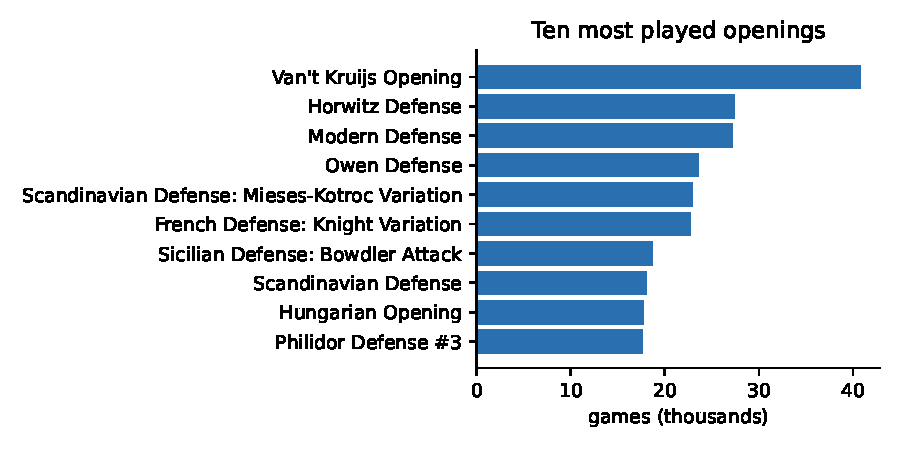
\includegraphics[width=0.58\linewidth]{top_openings}\hfill
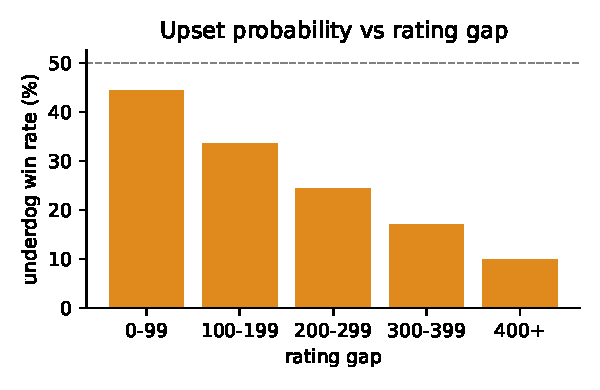
\includegraphics[width=0.38\linewidth]{upsets}
\caption{Left: ten most played openings (DataFrame). Right: upset probability by rating gap.}
\end{figure}
\begin{figure}[H]\centering
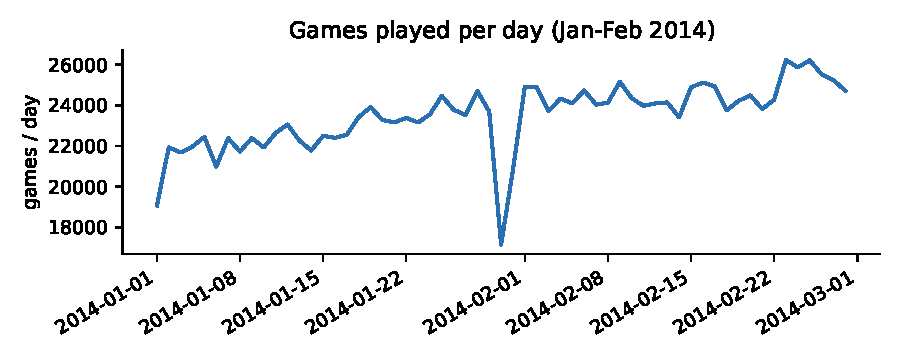
\includegraphics[width=0.49\linewidth]{daily_games}\hfill
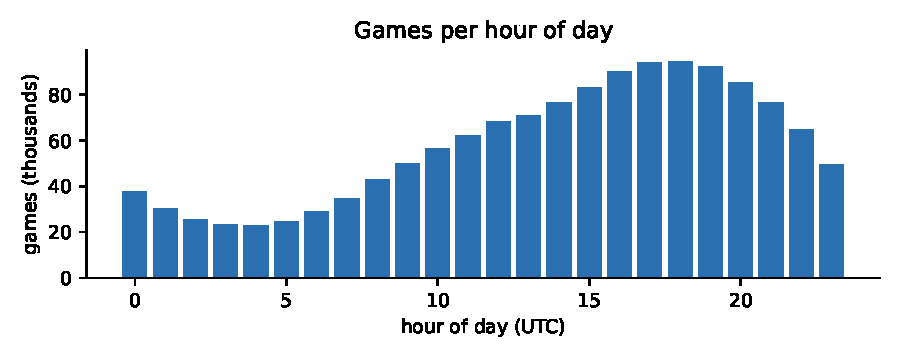
\includegraphics[width=0.49\linewidth]{hourly_games}
\caption{Monthly trend (games per day) and daily cycle (games per UTC hour).}
\end{figure}

\textbf{Other queries} (all saved under \texttt{results/}): most played openings with white
score (e.g.\ Scandinavian Mieses-Kotroc 60.4\% for white versus Sicilian Bowdler Attack
43.5\%), top players by games with win rate (one prolific account, \texttt{houdjini},
scores 85.5\% over 3,594 games at average rating 2231), ECO volume (volumes C and D favour
white at 54\%), and top terms (castling \texttt{O-O} is the most frequent token).

\textbf{Observations.}
\begin{enumerate}\itemsep0pt
\item Bullet is the fastest and its players are strongest on average (1673), yet 57\% of
bullet games end on the clock, against 15--17\% for Rapid and Classical.
\item Game length grows with rating (51 plies at 1000 to 84 at 2200) and so does the
draw rate (2.8\% $\rightarrow$ 6.3\%): stronger players blunder less.
\item The Elo model is visible in the data: upset probability falls smoothly with the
rating gap, from 44\% to 10\%, as the model predicts.
\item Traffic peaks at 18:00 UTC (94.4k games) and bottoms at 04:00 (23.0k), a 4$\times$
daily swing; weekends are only slightly busier (24.3k on Sunday vs 22.8k on Thursday).
\item The RDD counts (Table~2) and DataFrame counts differ slightly
(e.g.\ Van't Kruijs 41,190 vs 40,808) because the DataFrame numbers are taken after cleaning.
\end{enumerate}

%------------------------------------------------------------------
\section{Analytics Workflow (Part D)}\label{sec:workflow}
\texttt{part\_d\_pipeline.py} wires the two APIs together exactly as in the required
workflow; Figure~\ref{fig:wf} shows it with the measured wall time of every stage.

\begin{figure}[H]\centering
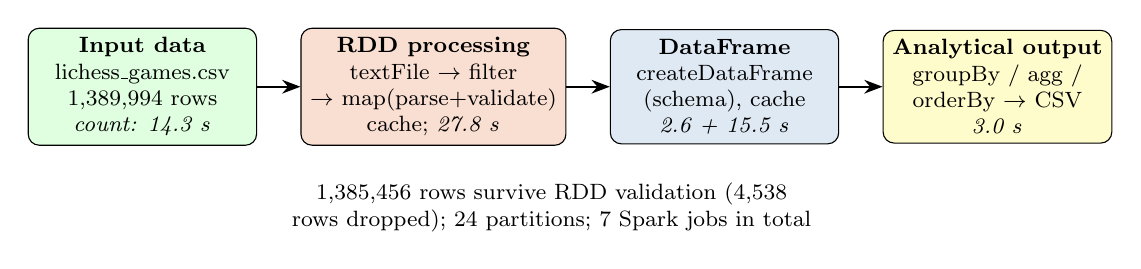
\begin{tikzpicture}[font=\footnotesize,node distance=0.55cm,
  st/.style={draw,rounded corners,align=center,minimum width=2.9cm,minimum height=1.35cm,fill=gray!8},
  arr/.style={-{Stealth},thick}]
\node[st,fill=green!12] (in) {\textbf{Input data}\\lichess\_games.csv\\1,389,994 rows\\\emph{count: 14.3 s}};
\node[st,right=of in,fill=sparkorange!20] (rdd) {\textbf{RDD processing}\\textFile $\rightarrow$ filter\\$\rightarrow$ map(parse+validate)\\cache; \emph{27.8 s}};
\node[st,right=of rdd,fill=blue1!15] (df) {\textbf{DataFrame}\\createDataFrame\\(schema), cache\\\emph{2.6 + 15.5 s}};
\node[st,right=of df,fill=yellow!20] (out) {\textbf{Analytical output}\\groupBy / agg /\\orderBy $\rightarrow$ CSV\\\emph{3.0 s}};
\draw[arr] (in)--(rdd); \draw[arr] (rdd)--(df); \draw[arr] (df)--(out);
\node[below=0.35cm of rdd,xshift=1.5cm,align=center,text width=8cm] {1,385,456 rows survive RDD validation (4,538 rows dropped); 24 partitions; 7 Spark jobs in total};
\end{tikzpicture}
\caption{Spark analytics workflow with measured stage times (one local machine).}\label{fig:wf}
\end{figure}

The pipeline's output is the ten opening/time-control combinations (at least 500 games)
with the highest white score: Barnes Defense in blitz (0.851, 583 games) and
King's Knight Opening in bullet (0.734) lead; such lines are mostly played at lower
ratings (mean 1328 for the Barnes Defense games), where one-sided results are common. The dataflow shows the usual Spark trade-off:
the RDD stage is the most expensive because Python lambdas and the \texttt{csv} module run
row by row, while DataFrame operations (3.0 s over 1.39M rows) run in the JVM with
Catalyst-optimised physical plans (\texttt{HashAggregate} $\rightarrow$ \texttt{Exchange}
$\rightarrow$ \texttt{HashAggregate} with a partial aggregation before the shuffle).

%------------------------------------------------------------------
\section{Streaming (Part E)}\label{sec:stream}
\textbf{Stream source.} A producer thread acts as the Lichess game feed: it listens on a
local TCP socket and pushes one burst of 10,000 tab-separated game records every
3 seconds, 20 bursts in total (200,000 games, 20$\times$ the required 10k).

\textbf{Processing.} Spark cuts the feed into 3-second micro-batches. For every batch we
(i)~\emph{count the records} and summarise white/black wins, draws and mean rating,
(ii)~keep running totals per termination type (stateful aggregation), and
(iii)~compute a sliding 9-second window count per termination type
(\texttt{reduceByKeyAndWindow}).

\begin{table}[H]\centering\small
\caption{Selected micro-batches (all 19 are in \texttt{results/e\_stream\_batches.csv}).}
\begin{tabular}{@{}rrrrrr@{}}\toprule
Batch & Records & White wins & Black wins & Draws & Mean rating\\\midrule
1 & 10,000 & 5,199 & 4,482 & 319 & 1628.0\\
2 & 10,000 & 5,072 & 4,599 & 329 & 1628.5\\
9 & 10,000 & 5,169 & 4,536 & 295 & 1591.0\\
18 & 20,000 & 10,222 & 9,210 & 568 & 1614.5\\
19 & 10,000 & 5,132 & 4,585 & 283 & 1615.1\\\midrule
\textbf{Total (19 batches)} & \textbf{200,000} & & & &\\\bottomrule
\end{tabular}\end{table}

\begin{figure}[H]\centering
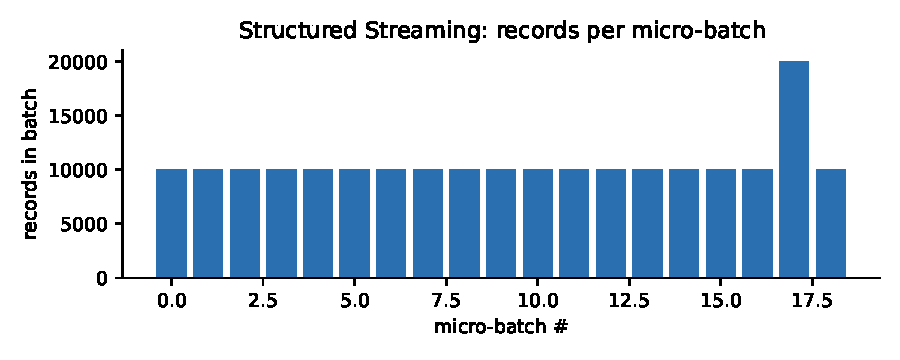
\includegraphics[width=0.49\linewidth]{stream_batches}\hfill
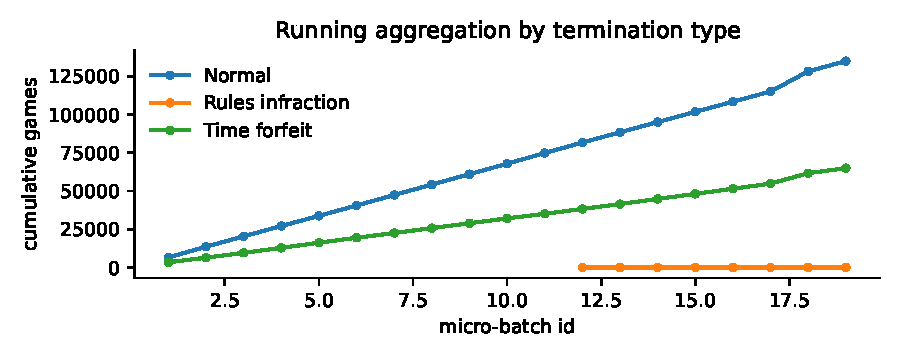
\includegraphics[width=0.49\linewidth]{stream_running}
\caption{Left: records counted per micro-batch. Right: running totals by termination type;
after 200,000 games: Normal 134,978, Time forfeit 64,968, Rules infraction 54.}
\end{figure}

\textbf{Results.} All 200,000 records were processed with none lost. Per-batch statistics are
stable (white wins 50.7--52.7\%, mean rating 1591--1630), because the replay order is
chronological; the running termination mix converges to 67.5\% Normal / 32.5\% Time forfeit,
matching the 1.39M-game figures of Section~\ref{sec:df} closely (67.0\% / 33.0\%), an
illustration of how a stream sample estimates the whole. Batches completed about
9--10~s apart instead of 3~s: processing took longer than the batch interval on this
4-thread local setup (one thread is occupied by the receiver), so bursts queued in the socket
buffer and batch~18 contains two bursts. This is back-pressure; more executors would
mitigate it.

\textbf{Honest limitation: Structured Streaming.} The assignment names Structured Streaming.
We wrote it (\texttt{part\_e\_structured\_streaming.py}: socket source, \texttt{foreachBatch}
per-batch aggregation, a complete-mode running aggregate) but \textbf{could not run it}:
every Structured Streaming query creates checkpoint directories through Hadoop's file
system layer, which on Windows needs the native \texttt{winutils.exe} and \texttt{hadoop.dll};
only the former could be emulated locally. The reported results therefore come from the
equivalent classic Spark Streaming (DStream) micro-batch API, which needs no checkpoint
for these operations. The conceptual model is the same (an unbounded table processed in
micro-batches); the Structured version should run unchanged on Linux, WSL or Docker.

\textbf{Sampling and filtering in a stream.} The stream here is the sequence of games as
they finish. Filtering is done on the fly (malformed lines are dropped in
\texttt{filter}); sampling (e.g.\ every $k$-th game or a reservoir of fixed size) would let
a downstream consumer maintain estimates such as the termination mix with constant memory.

%------------------------------------------------------------------
\section{Results and Discussion}
\begin{itemize}\itemsep1pt
\item \textbf{Scale.} 1.39M games / 93.3M tokens processed locally; RDD jobs in minutes,
DataFrame queries in seconds. The RDD jobs took minutes and the DataFrame stage seconds
(not a like-for-like comparison, but consistent with JVM-side execution and
Catalyst's partial aggregation versus per-row Python lambdas).
\item \textbf{Domain insights.} White advantage $\approx$2.5 points; time controls change
how games end (57\% clock losses in bullet); strength reduces blunders (longer games, more
draws); Elo-predicted upset rates hold across 1.39M games; a strong diurnal cycle with a 4$\times$
peak-to-trough ratio.
\item \textbf{Data quality.} 0.33\% of rows needed removal, mostly correspondence games
without a clock.
\item \textbf{Limits.} Local mode only (no multi-node speed-up measured); two months of
2014 data, so statements concern early-Lichess, not modern play; ratings are from the
platform's own system; the streaming results come from the DStream API (Section~\ref{sec:stream}).
\end{itemize}

%------------------------------------------------------------------
\section{Conclusion}
We built and executed an end-to-end Spark pipeline over 1.39 million real chess games:
architecture and environment (A), RDD transformations and actions (B), DataFrame cleaning,
aggregation and SQL (C), a measured RDD$\rightarrow$DataFrame workflow (D), and a
200,000-record micro-batch stream with per-batch, running and windowed aggregation (E). The
analysis recovered known chess regularities from data alone, which also validates the
pipeline. The remaining gap is running the Structured Streaming script on a platform with
Hadoop native support and benchmarking on a multi-node cluster; both are mechanical
given the code provided.

\section*{References}
\begin{small}\begin{enumerate}\itemsep1pt
\item Lichess.org Open Database. \url{https://database.lichess.org} (CC0).
\item M.~Zaharia et al. \emph{Resilient Distributed Datasets: A Fault-Tolerant Abstraction
for In-Memory Cluster Computing.} NSDI 2012.
\item M.~Armbrust et al. \emph{Spark SQL: Relational Data Processing in Spark.} SIGMOD 2015.
\item M.~Armbrust et al. \emph{Structured Streaming: A Declarative API for Real-Time
Applications in Apache Spark.} SIGMOD 2018.
\item M.~Zaharia et al. \emph{Discretized Streams: Fault-Tolerant Streaming Computation at
Scale.} SOSP 2013.
\item J.~Dean and S.~Ghemawat. \emph{MapReduce: Simplified Data Processing on Large
Clusters.} OSDI 2004.
\item A.~Elo. \emph{The Rating of Chessplayers, Past and Present.} Arco, 1978.
\item Apache Spark documentation, version 3.5. \url{https://spark.apache.org/docs/3.5.3/}
\end{enumerate}\end{small}
\end{document}
